\tocsection{\textbf{10/19/26 Lecture 23:} Contractible Spaces, Retractions, and Simplicial Complexes}

Recall that if two path connected spaces are homotopy equivalent, they have isomorphic fundamental groups.

\begin{lemma}[\textbf{Corollary 23.1}]
    If $n > 2$, then $\R^2$ is not homeomorphic to $\R^n$.
\end{lemma}
\begin{proof}{Proof:}
    Say $f : \R^2 \to \R^n$ is a homeomorphism. Then, $f\res{\R^2 - \{0\}} : \R^2 \setminus \{0\} \to \R^n \setminus \{f(0)\}$ is a homeomorphism, and so it is a homotopy equivalence.\\

    Hence $\pi_1(\R^2 - \{0\})$ is isomorphic to $\pi_1(\R^n \setminus \{f(0)\})$.\\

    Now, $\R^2 - \{0\}$ deformation retracts to $S^1$ and $\R^n \setminus \{f(0)\}$ deformation retracts to a sphere $S^{n - 1}$ around $f(0)$.\\

    Since fundamental groups are invariant under deformation retracts, we have
    \[ \pi_1(\R^2 \setminus \{0\}) = \pi_1(S^1) = \Z \]
    and
    \[ \pi_1(\R^n \setminus \{f(0)\}) = \pi_1(S^{n - 1}) = \{e\} \]
    as $n - 1 > 1$. This is a contradiction.

    $\qed$
\end{proof}

\begin{definition}[\textbf{Definition 23.2:} Contractible Spaces]
    We say $X$ is \emph{contractible} if $\id_X$ is homotopic to a constant map $c_p : X \to \{p\}$.
\end{definition}

\begin{lemma}[\textbf{Proposition 23.3}]
    The following are true about contractible spaces:
    \begin{enumerate}[label=\alph*.]
        \item $X$ is contractible if, and only if, $X$ is homotopy equivalent to a point.
        \item $X$ is contractible $\implies$ $X$ is simply connected.
        \item If $X$ is contractible, then any two maps $f, g : Z \to X$ are homotopic.
        \item If $X$ is contractible, then $\id_X \simeq c_x$ for any $x \in X$.
    \end{enumerate}
\end{lemma}
\begin{proof}{Proof:}
    \textbf{a)} $(\Rightarrow)$ Say $\alpha_p : X \to \{p\}$ is the map and $i_p : \{p\} \hookrightarrow X$ is the inclusion.
    \begin{center}
        \begin{tikzcd}
            X \arrow[r, bend left, pos = 0.6, "\alpha_p"] & \{p\} \arrow[l, bend left, pos = 0.4, "i_p"]
        \end{tikzcd}
    \end{center}
    Now, $\alpha_p \circ i_p = \id_p$ and $i_p \circ \alpha_p = c_p \simeq \id_X$. Thus, $X$ is homotopy equivalent to $\{p\}$.\\

    $(\Leftarrow)$ Suppose $X$ is homotopy equivalent to a point $\{p\}$. Then, we have $f : X \to \{p\}$ and $g : \{p\} \to X$ such that
    \[ f \circ g \simeq \id_{\{p\}} \quand g \circ f \simeq \id_X \]
    However, $g \circ f = c_{g(p)}$, so $\id_X \simeq c_{g(p)}$, so $X$ is contractible.\\

    \textbf{b)} Suppose $X$ is contractible. Now, $\id_X \simeq c_p$, so there exists $F : X \times I \to X$ such that $F(x, 0) = x$ and $F(x, 1) = p$. Now, given $y \in X$, take $\gamma(t) = F(y, t)$. We see $\gamma$ is a path from $y$ to $p$. Thus, $X$ is path connected ($p$ connects to all points).\\

    Now, since $X$ is homotopy equivalent to $\{p\}$, and as $\pi_1(X) \simeq \pi_1(p) \simeq \{e\}$, we see $X$ is simply connected.\\

    \textbf{c)} Suppose $X$ is contractible. Then, $\id_X \simeq c_p$. Thus,
    \begin{align*}
        f &\simeq \id_X \circ f \simeq c_p \circ f\\
        g &\simeq \id_X \circ g \simeq c_p \circ g
    \end{align*}
    but $c_p \circ f$ and $c_p \circ g$ are both the same map sending $Z \to \{p\}$. Thus, $f \simeq g$.\\

    \textbf{d)} Follows from (c) immediately.

    $\qed$
\end{proof}

\begin{definition}[\textbf{Definition 23.4:} Retractions]
    If $A \subseteq X$, a \emph{retraction} of $X$ to $A$ is a map $g : X \to A$ so $g\res{A} = \id_A$. We say $A$ is a \emph{retract} of $X$.
\end{definition}

\begin{example}{\textbf{Example:} Retraction to a Point}
    If $X = S^1$ and $A = \{1\}$, then the map $g : X \to A$ is a retraction.
\end{example}

\textbf{Note:} A deformation retraction gives a retraction $g(x) = G(x, 1)$.

\begin{lemma}[\textbf{Proposition 23.5}]
    If $g : X \to A$ is a retraction, then $g_{*} : \pi_1(X, a) \to \pi_1(A, a)$ is onto for $a \in A$. 
\end{lemma}
\begin{proof}{Proof:}
    Say $i : A \to X$ is the inclusion. Then $g \circ i = \id_A$, so $g_* \circ i_* = \id_{\pi_1(A, a)}$. Thus, $g_*$ must be onto. This can be seen below. 
    \begin{center}
        \begin{tikzcd}
            \pi_1(A, a) \arrow[r, "i_*"] \arrow[rr, bend right = 25, "\id_{\pi_1(A, a)}"'] & \pi_1(X, a) \arrow[r, "g_*"] & \pi_1(A, a)
        \end{tikzcd}
    \end{center}

    $\qed$
\end{proof}

\subsection*{Simplicial Complexes}
\sectionspace

These will be spaces built out of ``generalized triangles''.

\begin{definition}[\textbf{Definition 23.6:} Hyperplanes]
    Say $v_0, \ldots, v_k$ are points in $\R^n$. Then, the \emph{hyperplane} they span is
    \[ \{\lambda_0 v_0 + \lambda_1 v_1 + \cdots + \lambda_k v_k \col \lambda_0 + \cdots + \lambda_k = 1\} \]
    This is the same as
    \[ \{v_0 + r_1(v_1 - v_0) + \cdots + r_k(v_k - v_0) \col r_1, \ldots, r_k \in \R\} \]
\end{definition}

\textbf{Example:}
\fig{0.45}{Lecture23Fig1}{}

\begin{definition}[\textbf{Definition 23.7:} General Position]
    Let $H$ be the hyperplane formed by $v_0, \ldots, v_k$ in $\R^n$. We say $v_0, \ldots, v_k$ are in \emph{general position} if $\dim H = k$.
\end{definition}

\begin{definition}[\textbf{Definition 23.8:} Simplices]
    If $v_0, \ldots, v_k$ are in general position, then the smallest convex set containing them, called the \emph{convex hull}, is the set
    \[ C = \{\lambda_0 v_0 + \cdots + \lambda_k v_k \col \lambda_0 + \cdots + \lambda_k = 1, \lambda_0 \geq 0, \lambda_1 \geq 0, \ldots, \lambda_k \geq 0\} \]
    we call this the \emph{$k$-dimensional simplex} containing $v_0, \ldots, v_k$.
    \fig{0.4}{Lecture23Fig2}{}
\end{definition}

\begin{example}{\textbf{Example:} Low-Dimensional Simplices}
    If $k = 0$ we get a point, $k = 1$ a line, $k = 2$ a triangle, $k = 3$ a tetrahedron.
\end{example}

\begin{definition}[\textbf{Definition 23.9:} Faces]
    If $A$ and $B$ are simplices and $\{\tt{vertices of } B\} \subseteq \{\tt{vertices of } A\}$, then $B$ is a \emph{face} of $A$.
\end{definition}

\begin{example}{\textbf{Example:} Faces of a Triangle}
    If $A$ is a triangle, it has $7$ faces as there are $7$ nonempty subsets of $\{v_0, v_1, v_2\}$.
\end{example}

\begin{definition}[\textbf{Definition 23.10:} Simplicial Complexes]
    A finite collection of simplices in some $\R^n$ is a (finite) \emph{simplicial complex} $K$ if
    \begin{enumerate}
        \item When $A$ is a simplex in the collection, so are its faces.
        \item When two simplices intersect, they do so in a common face.
    \end{enumerate}
\end{definition}

\begin{center}
    \begin{minipage}{0.45\textwidth}
        \textbf{Example:}\\[0.2cm]
        \centering
        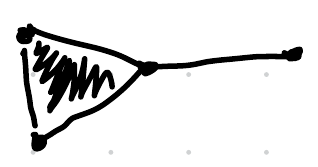
\includegraphics[scale = 0.45]{Lecture23Fig3}
    \end{minipage}
    \hfill
    \begin{minipage}{0.45\textwidth}
        \textbf{Non-Example:}\\[0.2cm]
        \centering
        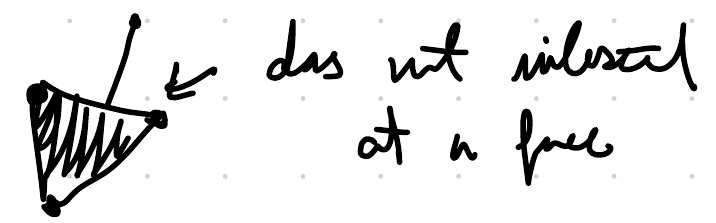
\includegraphics[scale = 0.45]{Lecture23Fig4}
    \end{minipage}
\end{center}

\begin{center}
    \begin{minipage}{0.45\textwidth}
        \textbf{Example:}\\[0.2cm]
        \centering
        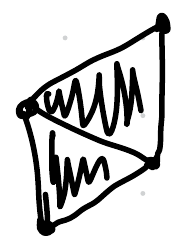
\includegraphics[scale = 0.45]{Lecture23Fig5}
    \end{minipage}
    \hfill
    \begin{minipage}{0.45\textwidth}
        \textbf{Non-Example:}\\[0.2cm]
        \centering
        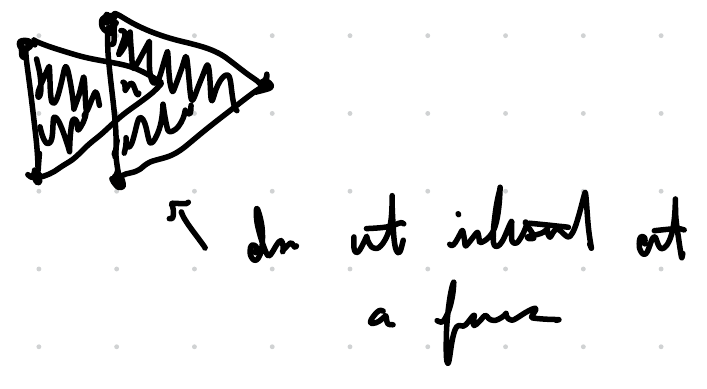
\includegraphics[scale = 0.45]{Lecture23Fig6}
    \end{minipage}
\end{center}

\textbf{Note:} A simplicial complex is a collection, so we write $\abs{K}$ for the corresponding subset of $\R^n$.
